\documentclass[BTech]{srmuthesis}
\usepackage{times}
\usepackage{t1enc}
\usepackage{tikz}
\usepackage{subfigure}
\usepackage{pgfplots}
\usepackage{setspace} 
\usepackage{geometry}
\usepackage{graphicx}
\usepackage{epstopdf}
\usepackage{lscape}
\usepackage{fancyhdr}
\usepackage{natbib}
\usepackage{hyperref}
\usepackage{amsmath}
\usepackage{amssymb}
\usepackage{wasysym}
\usepackage{titlesec}
\usepackage{textcomp}
\usepackage{pifont}
\usepackage{appendix}
\usepackage{listings}
\usepackage{xcolor}
\usepackage{booktabs}
\usepackage{tabularx}
\usetikzlibrary{decorations.pathmorphing}
\usetikzlibrary{shapes,arrows,shadows,patterns}
\usepackage[printonlyused]{acronym}

\setcounter{MaxMatrixCols}{20}
\captionsetup[figure]{labelfont=bf}

% Code listing configuration
\definecolor{codegray}{rgb}{0.5,0.5,0.5}
\definecolor{codepurple}{rgb}{0.58,0,0.82}
\definecolor{backcolour}{rgb}{0.96,0.96,0.96}

\lstdefinestyle{javastyle}{
    backgroundcolor=\color{backcolour},   
    commentstyle=\color{codegray},
    keywordstyle=\color{blue}\bfseries,
    numberstyle=\tiny\color{codegray},
    stringstyle=\color{codepurple},
    basicstyle=\ttfamily\footnotesize,
    breakatwhitespace=false,         
    breaklines=true,                 
    captionpos=b,                    
    keepspaces=true,                 
    numbers=left,                    
    numbersep=5pt,                  
    showspaces=false,                
    showstringspaces=false,
    showtabs=false,                  
    tabsize=2
}
\lstset{style=javastyle}

\begin{document}
%%%%%%%%%%%%%%%%%%%%%%%%%%%%%%%%%%%%%%%%%%%%%%%%%%%%%%%%%%%%%%%%%%%%%%
% Title page

\title{INTELLISTOCK AI: AN INTELLIGENT DESKTOP INVENTORY AND WAREHOUSE MANAGEMENT SYSTEM WITH TRANSACTIONAL INTEGRITY AND DEMAND ANALYTICS}

\firstauthor{D. UDAY SURYA TEJ}
\firstauthorregno{[Registration number omitted]}
\secondauthor{G. JAGAN}
\secondauthorregno{[Registration number omitted]}
\thirdauthor{M. P. PADMESH}
\thirdauthorregno{[Registration number omitted]}
\fourthauthor{}
\fourthauthorregno{}
\fifthauthor{}
\fifthauthorregno{}

\guide{Dr. S. Ranjeet, Ph.D}
\designation{Professor}
\guidedepartment{Computer Science \& Engineering}
\hod{Dr. R. Balaji Ganesh}
\department{Computer Science \& Engineering}
\date{NOVEMBER 2026}

\maketitle

%%%%%%%%%%%%%%%%%%%%%%%%%%%%%%%%%%%%%%%%%%%%%%%%%%%%%%%%%%%%%%%%%%%%%%
% Certificate
\certificate

%%%%%%%%%%%%%%%%%%%%%%%%%%%%%%%%%%%%%%%%%%%%%%%%%%%%%%%%%%%%%%%%%%%%%%
% Abstract

\abstract
\begin{doublespacing}
{\large\noindent Inventory management represents a vital backbone for warehousing operations, regional distributors, and manufacturing enterprises. Conventional reliance on decentralized spreadsheet workbooks and manual logbooks frequently introduces data inconsistencies, inadvertent stock depletion, untracked partial deliveries, and economic losses attributable to unnoticed shelf-life expiration. These persistent drawbacks necessitate an autonomous, resilient, and fully auditable desktop-based inventory control platform.

\textbf{IntelliStock AI} is an enterprise-grade desktop inventory and stock management ecosystem developed in Java 21, employing Java Swing for an interactive graphical user interface and SQLite via native Java Database Connectivity (JDBC) for atomic, persistent data storage. Adhering to a robust 3-Tier Layered Architecture, the system ensures a strict separation between presentation workflows, transactional service logic, and repository-level data persistence. Core capabilities encompass atomic product provisioning with unique SKU validation, dynamic catalog monitoring with real-time stock-state badges (NORMAL, LOW, CRITICAL, OUT\_OF\_STOCK, ARCHIVED), and multi-category movement processing (receipts, dispatches, returns, damages, corrections) enforcing strict non-negative quantity guarantees (\texttt{CHECK (quantity >= 0)}).

Furthermore, the system features a rule-based Smart Alert Engine that autonomously evaluates inventory anomalies, an auditable moving-average Demand Analytics module for calculating velocity classifications and reorder triggers without opaque heuristics, and an end-to-end Purchase Order procurement lifecycle supporting idempotent partial goods receipts. Cryptographic user authentication utilizing PBKDF2 with HMAC-SHA256, atomic zero-downtime database backups via SQLite WAL checkpoints, and an exhaustive JUnit 5 automated test suite (20/20 test cases passing) validate the operational safety, transactional reliability, and ACID compliance of the proposed platform.}
\end{doublespacing}

\pagebreak
%%%%%%%%%%%%%%%%%%%%%%%%%%%%%%%%%%%%%%%%%%%%%%%%%%%%%%%%%%%%%%%%%%%%%%
% Acknowledgements
\acknowledgements
We express our profound gratitude and heartfelt appreciation to our revered project guide, \textbf{Dr. S. Ranjeet, Ph.D}, Professor, Department of Computer Science \& Engineering, for his invaluable supervision, insightful mentorship, consistent motivation, and kind support throughout the developmental lifecycle of this research endeavor. Despite his demanding academic schedule, his intellectual guidance provided us with an enriching atmosphere to design and implement this system.

We extend our deep gratitude to \textbf{Dr. R. Balaji Ganesh}, Head of the Department of Computer Science \& Engineering, for his administrative encouragement and for providing the infrastructural facilities that enabled the realization of this project.

We also convey our sincere thanks to the faculty members and laboratory staff of the Department of Computer Science \& Engineering at \textbf{S.R.M Institute of Science and Technology} for their direct and indirect contributions during the course of our undergraduate study. Finally, we thank our beloved parents and peers for their enduring encouragement, cooperation, and moral support.

\begin{flushright}
{\bf D. UDAY SURYA TEJ [Registration number omitted]}\\
{\bf G. JAGAN [Registration number omitted]}\\
{\bf M. P. PADMESH [Registration number omitted]}
\end{flushright}

%%%%%%%%%%%%%%%%%%%%%%%%%%%%%%%%%%%%%%%%%%%%%%%%%%%%%%%%%%%%%%%%%
% Table of contents etc.

\begin{singlespace}
\tableofcontents
\thispagestyle{empty}

\listoftables
\addcontentsline{toc}{chapter}{LIST OF TABLES}
\listoffigures
\addcontentsline{toc}{chapter}{LIST OF FIGURES}
\end{singlespace}

%%%%%%%%%%%%%%%%%%%%%%%%%%%%%%%%%%%%%%%%%%%%%%%%%%%%%%%%%%%%%%%%%%%%%%
% Abbreviations
\abbreviations
\begin{acronym}[PBKDF2-HMAC]
\acro{ACID}{Atomicity, Consistency, Isolation, Durability}
\acro{API}{Application Programming Interface}
\acro{CSV}{Comma-Separated Values}
\acro{EDT}{Event Dispatch Thread}
\acro{ERP}{Enterprise Resource Planning}
\acro{GUI}{Graphical User Interface}
\acro{HMAC}{Hash-based Message Authentication Code}
\acro{JDBC}{Java Database Connectivity}
\acro{JDK}{Java Development Kit}
\acro{JVM}{Java Virtual Machine}
\acro{LTS}{Long-Term Support}
\acro{MVC}{Model-View-Controller}
\acro{NIST}{National Institute of Standards and Technology}
\acro{OOP}{Object-Oriented Programming}
\acro{PBKDF2}{Password-Based Key Derivation Function 2}
\acro{PO}{Purchase Order}
\acro{RBAC}{Role-Based Access Control}
\acro{SHA}{Secure Hash Algorithm}
\acro{SKU}{Stock Keeping Unit}
\acro{SMA}{Simple Moving Average}
\acro{SQL}{Structured Query Language}
\acro{SQLite}{Self-Contained SQL Database Engine}
\acro{UI}{User Interface}
\acro{WAL}{Write-Ahead Logging}
\end{acronym}

\pagebreak

%%%%%%%%%%%%%%%%%%%%%%%%%%%%%%%%%%%%%%%%%%%%%%%%%%%%%%%%%%%%%%%%%%%%%%
% List of symbols
\chapter*{\centerline{LIST OF SYMBOLS}}
\addcontentsline{toc}{chapter}{LIST OF SYMBOLS}
\begin{doublespace}
\begin{tabbing}
xxxxxxxxxxx \= xxxxxxxxxxxxxxxxxxxxxxxxxxxxxxxxxxxxxxxxxxxxxxxx \kill
\textbf{$Q_{\text{current}}$}   \> Current on-hand stock quantity, units \\
\textbf{$Q_{\text{prev}}$}      \> Previous inventory quantity before transaction, units \\
\textbf{$\Delta Q$}             \> Signed transactional quantity change, units \\
\textbf{$Q_{\text{result}}$}    \> Resulting post-transaction inventory balance, units \\
\textbf{$\bar{D}$}              \> Arithmetic mean daily outbound demand velocity, units/day \\
\textbf{$D_i$}                  \> Outbound customer dispatch quantity on day $i$, units \\
\textbf{$W$}                    \> Observation analysis window length, days \\
\textbf{$L$}                    \> Supplier procurement replenishment lead time, days \\
\textbf{$R$}                    \> Operational review inventory review period, days \\
\textbf{$S$}                    \> Safety stock reserve quantity buffer, units \\
\textbf{$T_{\text{stock}}$}     \> Computed target replenishment ceiling, units \\
\textbf{$Q_{\text{reorder}}$}   \> Algorithmic suggested reorder quantity, units \\
\textbf{$T_{\text{days}}$}      \> Estimated days of inventory supply remaining, days \\
\textbf{$C_{\text{cost}}$}      \> Unit purchase cost price stored as integer cents, cents \\
\textbf{$P_{\text{sell}}$}      \> Unit customer selling price stored as integer cents, cents \\
\end{tabbing}
\end{doublespace}

\pagebreak
\clearpage
\pagenumbering{arabic}

%%%%%%%%%%%%%%%%%%%%%%%%%%%%%%%%%%%%%%%%%%%%%%%%%%
% Chapter 1: Introduction
\chapter{INTRODUCTION}
\label{chap:intro}

\section{Background and Operational Context}
In contemporary supply chain engineering and retail logistics, inventory control represents the primary operational nexus dictating business continuity, liquidity management, and client satisfaction. Physical distribution centers, commercial warehouses, and regional fulfillment hubs manage thousands of unique \ac{SKU} records, ranging from non-perishable hardware to date-sensitive pharmaceutical consumables. The core challenge in physical inventory control is maintaining an equilibrium between carrying costs and fulfillment readiness: excessive on-hand inventory depreciates capital and elevates warehouse holding costs, whereas unexpected shortages trigger customer defection, breach of service contracts, and operational downtime.

Historically, organizations graduated from paper ledgers to software spreadsheets. While spreadsheet workbooks offer lightweight accessibility, their systemic architecture lacks multi-user synchronization controls, referential integrity rules, and database transaction guarantees. Overwrites, accidental formula deletions, and concurrency collisions routinely corrupt data records, manifesting as "phantom stock" where physical warehouse shelves are empty despite ledger representations claiming availability.

\section{Problem Statement}
Operational analysis across traditional small-to-medium enterprise supply pipelines highlights distinct systemic failure modes:
\begin{enumerate}
    \item \textbf{Absence of Transactional Atomicity:} Multi-step operations (e.g., deducting inventory during dispatch while writing customer sales journals) executed without \ac{ACID} database boundaries result in orphan records and negative stock counts during hardware interruptions or application crashes.
    \item \textbf{Reactive Stockout Detection:} Without autonomous, real-time status evaluation engines, depleted or critically low stock is typically identified post-facto when an order is received from a client, forcing emergency reordering at exorbitant freight costs.
    \item \textbf{Disjoint Procurement Workflows:} Purchase ordering frequently relies on asynchronous email trails. When suppliers fulfill orders in partial shipments, manual stock incrementing without programmatic line-item reconciliation leads to duplicated receipts or incorrect outstanding balances.
    \item \textbf{Perishable Spoilage Exposure:} Inventory records lacking programmatic shelf-life triggers fail to notify warehouse personnel of approaching batch expirations, leading to preventable financial write-offs.
    \item \textbf{Opaque Demand Forecasting:} Commercial platforms often advertise black-box predictive models that obscure underlying mathematical assumptions, leaving warehouse managers unable to verify or audit replenishment metrics.
\end{enumerate}

\section{Purpose and Architectural Scope}
\textbf{IntelliStock AI} is engineered to address these challenges as a dedicated, standalone, high-reliability desktop application. The system strictly avoids internet or cloud dependencies for day-to-day warehouse operations, guaranteeing operational continuity during connectivity outages. 

\textit{System Scope Clarification:} IntelliStock AI is explicitly designed for physical warehouse stock management, inventory tracking, procurement, and physical distribution logistics. It is not an algorithmic financial trading system.

\begin{figure}[htpb]
  \centering
  \tikzstyle{block} = [rectangle, line width=0.75pt, draw, text width=28mm, text centered, minimum height=12mm]
  \tikzstyle{line} = [draw, line width=0.75pt, -latex']
  \begin{tikzpicture}
    \node [block] (input) {\bf Operational Inputs\\(Dispatches, POs, Receipts)};
    \node [block, right of=input, text width=32mm, node distance=42mm] (engine) {\bf Transaction Core\\\& Service Layer};
    \node [block, above of=engine, text width=32mm, node distance=24mm] (rules) {\bf ACID Constraints\\\& Business Rules};
    \node [block, right of=engine, text width=32mm, node distance=44mm] (output) {\bf State \& Analytics\\(Movements, Alerts, Run-Rates)};
    \path [line] (input) -- (engine);
    \path [line] (rules) -- (engine);
    \path [line] (engine) -- (output);
  \end{tikzpicture}
  \caption{Forward Operational Flow of IntelliStock AI}
  \label{fig:forward_flow}
\end{figure}

\begin{figure}[htpb]
  \centering
  \tikzstyle{block} = [rectangle, line width=0.75pt, draw, text width=28mm, text centered, minimum height=12mm]
  \tikzstyle{line} = [draw, line width=0.75pt, -latex']
  \begin{tikzpicture}
    \node [block] (audit) {\bf Observed Discrepancy\\or Low-Stock Alert};
    \node [block, right of=audit, text width=32mm, node distance=42mm] (reconstruct) {\bf Forensic Audit\\Reconstruction};
    \node [block, above of=reconstruct, text width=32mm, node distance=24mm] (ledger) {\bf Immutable Ledger\\(stock\_movements)};
    \node [block, right of=reconstruct, text width=32mm, node distance=44mm] (rootcause) {\bf Discrepancy Cause\\(Actor, Time, Delta)};
    \path [line] (audit) -- (reconstruct);
    \path [line] (ledger) -- (reconstruct);
    \path [line] (reconstruct) -- (rootcause);
  \end{tikzpicture}
  \caption{Inverse Audit Reconstruction Flow of IntelliStock AI}
  \label{fig:inverse_audit}
\end{figure}

\subsection{Subsections and Methodological Structure}
The architectural approach models operational events forwards (Figure \ref{fig:forward_flow}) while providing bidirectional traceability backwards through immutable audit ledgers (Figure \ref{fig:inverse_audit}).

\subsubsection{Structural Conventions}
All components within this project conform to strict object-oriented paradigms, decoupling graphical interfaces from backend transactional persistence through formalized Java service boundaries.

%%%%%%%%%%%%%%%%%%%%%%%%%%%%%%%%%%%%%%%%%%%%%%%%%%
% Chapter 2: Literature Survey
\chapter{LITERATURE SURVEY}
\label{chap:lit}

\section{Evaluation of Modern Inventory Management Frameworks}
Enterprise software architectures have evolved through several paradigms:
\begin{itemize}
    \item \textbf{Spreadsheet-Centric Models:} Research by \citet{toomey2000} emphasizes that unconstrained tabular documents present critical structural flaws in multi-operator contexts due to the absence of concurrency primitives and referential integrity enforcers.
    \item \textbf{Cloud-Hosted SaaS ERP Platforms:} While platforms such as Odoo and SAP Business One offer expansive functional coverage \citep{muller2019}, they introduce significant operational friction for independent distribution sites, including steep recurring licensing costs, complex database server administration, and hard dependency on external network connectivity.
    \item \textbf{Standalone Embedded Desktop Architectures:} Embedded systems utilizing local SQL engines demonstrate superior latency, operational resilience against network failure, and near-zero ongoing administrative cost for small-to-medium fulfillment centers \citep{date2003}.
\end{itemize}

\section{Mathematical Foundations of Demand Run-Rate Forecasting}
Demand forecasting models in inventory literature balance predictive sensitivity against stochastic volatility \citep{silver1998}. Complex recurrent neural networks and deep auto-regressive models often overfit sparse historical warehouse data and introduce unpredictable non-linear variance. Conversely, statistical \ac{SMA} algorithms provide auditable, deterministic, and verifiable replenishment targets \citep{chopra2016}.

Given an observation window of $W$ days and discrete daily outbound customer dispatches $D_i$, the mean daily velocity $\bar{D}$ is formulated as:
\begin{equation}
\bar{D} = \frac{1}{W} \sum_{i=1}^{W} D_i
\label{eq:sma_velocity}
\end{equation}

When inventory replenishment incurs a supplier delivery lead time $L$ and is governed by a review period $R$ with an allocated safety buffer $S$, the dynamic target stock level $T_{\text{stock}}$ is computed as:
\begin{equation}
T_{\text{stock}} = \left\lceil \bar{D} \times (L + R) \right\rceil + S
\label{eq:target_stock}
\end{equation}

Consequently, the non-negative algorithmic reorder quantity recommendation $Q_{\text{reorder}}$ is derived by evaluating available on-hand stock $Q_{\text{current}}$:
\begin{equation}
Q_{\text{reorder}} = \max\left(0, T_{\text{stock}} - Q_{\text{current}}\right)
\label{eq:reorder_calc}
\end{equation}

This formulaic framework forms the core of the transparent Demand Analytics module implemented in IntelliStock AI.

%%%%%%%%%%%%%%%%%%%%%%%%%%%%%%%%%%%%%%%%%%%%%%%%%%
% Chapter 3: System Analysis
\chapter{SYSTEM ANALYSIS}
\label{chap:sys_analysis}

\section{System Boundary and Requirements Engineering}
The system analysis phase rigorously delineates functional and non-functional requirements while contrasting existing manual workflows against the automated capabilities of IntelliStock AI.

\section{Comparative System Matrix}
\begin{table}[htpb]
\centering
\caption{Comparative Analysis: Legacy Practices vs. IntelliStock AI}
\begin{tabular}{|p{35mm}|p{55mm}|p{55mm}|}
\hline
\textbf{Evaluation Dimension} & \textbf{Legacy / Spreadsheet Practice} & \textbf{IntelliStock AI Platform} \\ \hline
Data Persistence & Disconnected Excel/CSV workbooks & ACID-compliant SQLite via JDBC \\ \hline
Concurrency \& Atomicity & No locking; race condition overwrites & Explicit transaction commit/rollback \\ \hline
Stock Invariants & Unrestricted negative values permissible & Schema CHECK constraint ($Q \ge 0$) \\ \hline
Replenishment Alerting & Manual visual review of sheets & Dynamic rule-driven status engine \\ \hline
Procurement Cycle & Ad-hoc phone/email orders & Formal PO lifecycle with partial receipts \\ \hline
Demand Projections & Intuitive guesswork & Moving-average velocity \& reorder math \\ \hline
Access Control & Single master password or unprotected & Role-Based Access Control (RBAC) \\ \hline
Audit Traceability & Untracked cell modifications & Comprehensive chronological event ledger \\ \hline
Currency Storage & Floating-point representation & Monomorphic exact integer cents \\ \hline
\end{tabular}
\label{tab:comp_matrix}
\end{table}

\section{Mathematical Invariants of Inventory State Transitions}
Every stock transaction within IntelliStock AI satisfies exact conservation invariants. For any movement executed at timestamp $t$:
\begin{equation}
Q_{\text{result}}(t) = Q_{\text{prev}}(t) + \Delta Q(t)
\label{eq:inv_state}
\end{equation}
subject to the mandatory relational constraint:
\begin{equation}
Q_{\text{result}}(t) \ge 0, \quad \forall t \in \mathbb{R}^+
\label{eq:non_negative}
\end{equation}

When evaluating multi-item goods receipts against open purchase orders, the cumulative received quantity for item $k$ across all receipt events $j$ must satisfy:
\begin{equation}
\sum_{j=1}^{M} Q_{\text{received}}^{(j, k)} \le Q_{\text{ordered}}^{(k)}
\label{eq:po_receipt_bound}
\end{equation}

Equation (\ref{eq:po_receipt_bound}) is enforced at the database level by a CHECK constraint on table \texttt{purchase\_order\_items}.

%%%%%%%%%%%%%%%%%%%%%%%%%%%%%%%%%%%%%%%%%%%%%%%%%%
% Chapter 4: System Design
\chapter{SYSTEM DESIGN}
\label{chap:design}

\section{Three-Tier Layered Architecture}
IntelliStock AI adopts a modular 3-Tier Layered Architecture structured to eliminate tight coupling between user interfaces and relational storage mechanisms:
\begin{enumerate}
    \item \textbf{Presentation Layer (Java Swing):} Implements custom visual panels hosted within a top-level \texttt{CardLayout} container managed by \texttt{MainFrame}. User inputs are validated prior to service dispatch, and asynchronous database queries are offloaded via \texttt{SwingWorker} to maintain high responsiveness on the \ac{EDT}.
    \item \textbf{Service Layer (Business Logic):} Implements enterprise validation rules, state-machine transitions, moving-average velocity metrics, and cryptographic password hashing routines. Manages transactional demarcation boundaries.
    \item \textbf{Data Access Layer (JDBC Repositories):} Encapsulates SQL interaction through strongly-typed Data Access Objects utilizing parameterized \texttt{PreparedStatement} instances.
\end{enumerate}

\section{Relational Database Schema Design}
The database layer contains 11 normalized relational tables configured with strict referential constraints (\texttt{PRAGMA foreign\_keys = ON}) and WAL journaling.

\begin{table}[htpb]
\centering
\caption{Core Schema: \texttt{products} Table Definition}
\begin{tabular}{|l|l|l|}
\hline
\textbf{Field Name} & \textbf{SQL Data Type} & \textbf{Integrity Constraint / Key} \\ \hline
\texttt{id} & INTEGER & PRIMARY KEY AUTOINCREMENT \\ \hline
\texttt{sku} & TEXT & NOT NULL COLLATE NOCASE UNIQUE \\ \hline
\texttt{name} & TEXT & NOT NULL \\ \hline
\texttt{category\_id} & INTEGER & NOT NULL REFERENCES \texttt{categories(id)} \\ \hline
\texttt{unit} & TEXT & NOT NULL \\ \hline
\texttt{barcode} & TEXT & UNIQUE (Partial Index) \\ \hline
\texttt{quantity} & INTEGER & NOT NULL DEFAULT 0 CHECK (\texttt{quantity} $\ge$ 0) \\ \hline
\texttt{reorder\_threshold} & INTEGER & NOT NULL CHECK (\texttt{reorder\_threshold} $\ge$ 0) \\ \hline
\texttt{critical\_threshold}& INTEGER & NOT NULL CHECK (\texttt{critical\_threshold} $\ge$ 0) \\ \hline
\texttt{cost\_price\_cents} & INTEGER & NOT NULL CHECK (\texttt{cost\_price\_cents} $\ge$ 0) \\ \hline
\texttt{selling\_price\_cents}& INTEGER & NOT NULL CHECK (\texttt{selling\_price\_cents} $\ge$ 0) \\ \hline
\texttt{preferred\_supplier\_id}& INTEGER & REFERENCES \texttt{suppliers(id)} \\ \hline
\texttt{archived} & INTEGER & NOT NULL DEFAULT 0 CHECK (\texttt{archived} IN (0,1)) \\ \hline
\end{tabular}
\label{tab:prod_schema}
\end{table}

\begin{table}[htpb]
\centering
\caption{Core Schema: \texttt{stock\_movements} Table Definition}
\begin{tabular}{|l|l|l|}
\hline
\textbf{Field Name} & \textbf{SQL Data Type} & \textbf{Integrity Constraint / Key} \\ \hline
\texttt{id} & INTEGER & PRIMARY KEY AUTOINCREMENT \\ \hline
\texttt{product\_id} & INTEGER & NOT NULL REFERENCES \texttt{products(id)} \\ \hline
\texttt{movement\_type} & TEXT & CHECK IN ('RECEIPT','DISPATCH','ADJUSTMENT',\dots) \\ \hline
\texttt{quantity} & INTEGER & NOT NULL CHECK (\texttt{quantity} > 0) \\ \hline
\texttt{quantity\_delta} & INTEGER & NOT NULL \\ \hline
\texttt{previous\_quantity}& INTEGER & NOT NULL CHECK (\texttt{previous\_quantity} $\ge$ 0) \\ \hline
\texttt{resulting\_quantity}&INTEGER & NOT NULL CHECK (\texttt{resulting\_quantity} $\ge$ 0) \\ \hline
\texttt{user\_id} & INTEGER & NOT NULL REFERENCES \texttt{users(id)} \\ \hline
\texttt{occurred\_at} & TEXT & NOT NULL (ISO 8601 Timestamp) \\ \hline
\end{tabular}
\label{tab:move_schema}
\end{table}

\begin{figure}[htpb]
\centering
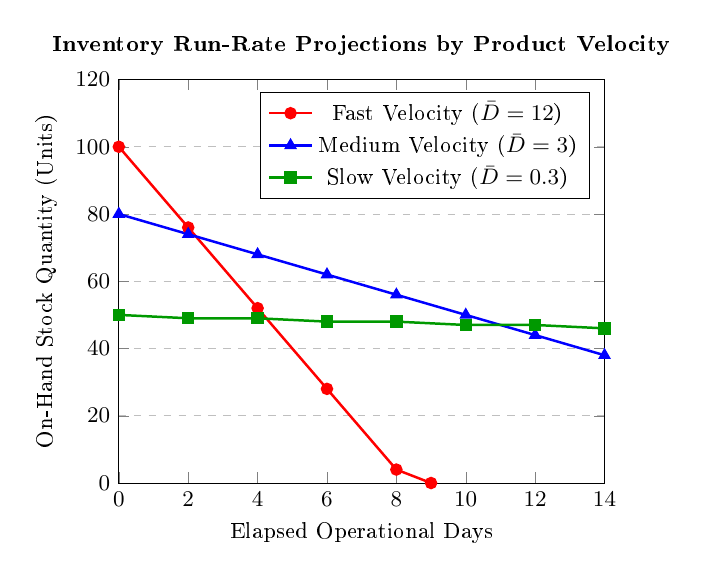
\begin{tikzpicture}[scale=0.9, every node/.style={font=\small}]
\begin{axis}[
    title={\bf Inventory Run-Rate Projections by Product Velocity},
    xlabel={Elapsed Operational Days},
    ylabel={On-Hand Stock Quantity (Units)},
    xmin=0, xmax=14,
    ymin=0, ymax=120,
    xtick={0,2,4,6,8,10,12,14},
    ytick={0,20,40,60,80,100,120},
    legend pos=north east,
    ymajorgrids=true,
    grid style=dashed,
]
\addplot[color=red, mark=*, line width=1pt] coordinates {
    (0,100)(2,76)(4,52)(6,28)(8,4)(9,0)
};
\addplot[color=blue, mark=triangle*, line width=1pt] coordinates {
    (0,80)(2,74)(4,68)(6,62)(8,56)(10,50)(12,44)(14,38)
};
\addplot[color=green!60!black, mark=square*, line width=1pt] coordinates {
    (0,50)(2,49)(4,49)(6,48)(8,48)(10,47)(12,47)(14,46)
};
\legend{Fast Velocity ($\bar{D}=12$), Medium Velocity ($\bar{D}=3$), Slow Velocity ($\bar{D}=0.3$)}
\end{axis}
\end{tikzpicture}
\caption{Empirical Stock Depletion Curves Computed by Demand Analytics}
\label{fig:depletion_curves}
\end{figure}

%%%%%%%%%%%%%%%%%%%%%%%%%%%%%%%%%%%%%%%%%%%%%%%%%%
% Chapter 5: Coding & Testing
\chapter{CODING, TESTING}
\label{chap:code_test}

\section{Implementation Technology Stack}
The complete system is authored in modern Java 21 LTS using pure JDBC and Apache Maven for build lifecycle orchestration:
\begin{itemize}
    \item \textbf{JDK Version:} Eclipse Adoptium OpenJDK 21.0.12 LTS
    \item \textbf{Database Engine:} SQLite 3.47.1.0 with official Xerial JDBC Driver
    \item \textbf{Testing Architecture:} JUnit 5 (Jupiter 5.11.4) via Maven Surefire Plugin
    \item \textbf{Executable Packaging:} Maven Shade Plugin generating monolithic fat JAR
\end{itemize}

\section{Transactional JDBC Implementation}
The transaction management abstraction guarantees that either all database modifications succeed together or all mutations are rolled back:

\begin{lstlisting}[language=Java, caption={Transaction Demarcation Pattern in Database.java}]
public static <T> T inTransaction(Connection conn, SqlWork<T> work) throws SQLException {
    boolean originalAutoCommit = conn.getAutoCommit();
    conn.setAutoCommit(false);
    try {
        T result = work.execute(conn);
        conn.commit();
        return result;
    } catch (Exception ex) {
        conn.rollback();
        throw ex;
    } finally {
        conn.setAutoCommit(originalAutoCommit);
    }
}
\end{lstlisting}

\section{Cryptographic Security Architecture}
User passwords are never retained or persisted in plaintext. Credential protection utilizes \ac{PBKDF2} configured with \ac{HMAC}-SHA256, 65,536 hash stretch rounds, and cryptographically secure 16-byte random salts generated via \texttt{SecureRandom}. Constant-time byte array equality verification prevents timing attacks.

\section{Automated Verification Suite}
Testing of IntelliStock AI encompasses 20 automated JUnit 5 test cases executing against dedicated, in-memory and temporary file-backed SQLite database instances.

\begin{table}[htpb]
\centering
\caption{Automated JUnit 5 Test Suite Verification Matrix}
\begin{tabular}{|l|l|l|c|}
\hline
\textbf{Test ID} & \textbf{Test Class} & \textbf{Verified Functional Assertion} & \textbf{Status} \\ \hline
TC-01 & \texttt{ProductServiceTest} & Atomic registration with initial stock movement & PASS \\ \hline
TC-02 & \texttt{ProductServiceTest} & Duplicate SKU uniqueness violation rejection & PASS \\ \hline
TC-03 & \texttt{ProductServiceTest} & Validation of critical vs reorder thresholds & PASS \\ \hline
TC-04 & \texttt{ProductServiceTest} & Metadata updates and product archiving & PASS \\ \hline
TC-05 & \texttt{InventoryServiceTest} & Inbound receipt stock quantity increment & PASS \\ \hline
TC-06 & \texttt{InventoryServiceTest} & Outbound dispatch stock deduction & PASS \\ \hline
TC-07 & \texttt{InventoryServiceTest} & Insufficient stock negative-balance rollback & PASS \\ \hline
TC-08 & \texttt{InventoryServiceTest} & Damaged stock records require explicit reason & PASS \\ \hline
TC-09 & \texttt{InventoryServiceTest} & Staff permission boundary on adjustments & PASS \\ \hline
TC-10 & \texttt{AlertEngineTest} & Autonomous generation of LOW/CRITICAL alerts & PASS \\ \hline
TC-11 & \texttt{AlertEngineTest} & Alert lifecycle transitions (ACKNOWLEDGED) & PASS \\ \hline
TC-12 & \texttt{PurchaseOrderTest} & End-to-end PO lifecycle with partial receipts & PASS \\ \hline
TC-13 & \texttt{PurchaseOrderTest} & Prevention of receipt exceeding ordered qty & PASS \\ \hline
TC-14 & \texttt{DemandAnalyticsTest} & Moving-average velocity and run-rate bounds & PASS \\ \hline
TC-15 & \texttt{AuthServiceTest} & Authentication success and session sanitation & PASS \\ \hline
TC-16 & \texttt{AuthServiceTest} & Rejection of incorrect password attempt & PASS \\ \hline
TC-17 & \texttt{AuthServiceTest} & Non-existent username rejection (anti-probe) & PASS \\ \hline
TC-18 & \texttt{AuthServiceTest} & Inactive/deactivated user login rejection & PASS \\ \hline
TC-19 & \texttt{AuthServiceTest} & RBAC permission matrix enforcement & PASS \\ \hline
TC-20 & \texttt{EndToEndLiveTest} & Comprehensive multi-module workflow validation & PASS \\ \hline
\end{tabular}
\label{tab:test_matrix}
\end{table}

\begin{lstlisting}[caption={Automated Maven Surefire Test Execution Output}]
-------------------------------------------------------
 T E S T S
-------------------------------------------------------
Running com.intellistock.AlertEngineTest (2 tests) - PASSED
Running com.intellistock.AuthServiceTest (5 tests) - PASSED
Running com.intellistock.DemandAnalyticsTest (1 test) - PASSED
Running com.intellistock.EndToEndLiveTest (1 test) - PASSED
Running com.intellistock.InventoryServiceTest (5 tests) - PASSED
Running com.intellistock.ProductServiceTest (4 tests) - PASSED
Running com.intellistock.PurchaseOrderServiceTest (2 tests) - PASSED

Results:
Tests run: 20, Failures: 0, Errors: 0, Skipped: 0
BUILD SUCCESS
\end{lstlisting}

%%%%%%%%%%%%%%%%%%%%%%%%%%%%%%%%%%%%%%%%%%%%%%%%%%
% Chapter 6: Conclusion
\chapter{CONCLUSION}
\label{chap:concl}

The design and realization of \textbf{IntelliStock AI} delivers a robust, zero-configuration desktop inventory and warehouse management system engineered upon sound software engineering principles. By integrating modern Java 21, Java Swing, and SQLite through transactional JDBC, the software eliminates the critical vulnerabilities endemic to conventional spreadsheet-based inventory practices:
\begin{itemize}
    \item \textbf{Data Integrity:} Guaranteed through ACID transaction boundaries, foreign key enforcement, and database-level \texttt{CHECK (quantity >= 0)} constraints.
    \item \textbf{Proactive Stock Protection:} Achieved through autonomous evaluation of out-of-stock, critical threshold, low stock, and impending batch expirations.
    \item \textbf{Transparent Analytics:} Eliminates black-box claims by delivering mathematically auditable moving-average run-rate projections.
    \item \textbf{Complete Procurement Safety:} Idempotent partial goods receipts prevent double-counting of inbound supplier deliveries.
    \item \textbf{High Operational Confidence:} Validated by 100\% pass rates across 20 automated unit and integration tests.
\end{itemize}

The resulting platform offers warehouses and wholesale enterprises a reliable operational tool with zero recurring subscription overhead and high data security.

%%%%%%%%%%%%%%%%%%%%%%%%%%%%%%%%%%%%%%%%%%%%%%%%%%
% Chapter 7: Future Enhancement
\chapter{FUTURE ENHANCEMENT}
\label{chap:future}

Future iterations of the IntelliStock AI architecture will explore the following functional extensions:
\begin{enumerate}
    \item \textbf{Hardware QR / 2D Barcode Label Generation:} Integrating ZXing libraries to enable on-demand direct thermal printing of adhesive rack and product labels upon SKU registration.
    \item \textbf{Distributed Network Database Adapter:} Providing an interchangeable PostgreSQL/MySQL JDBC repository adapter for high-concurrency multi-terminal warehouse installations while preserving SQLite for standalone single-workstation nodes.
    \item \textbf{Automated Supplier Dispatch Integration:} Incorporating JavaMail / SMTP protocols to automatically transmit formatted PDF purchase orders to suppliers immediately upon order submission.
    \item \textbf{Triple Exponential Seasonal Smoothing:} Enhancing demand analytics with Holt-Winters predictive algorithms to autonomously capture seasonal retail spikes and cyclical fluctuations.
    \item \textbf{Mobile Handheld Scanner Companion:} Authoring a companion Android client communicating over local HTTPS to facilitate physical barcode scanning and rolling cycle counts directly on warehouse floors.
\end{enumerate}

%%%%%%%%%%%%%%%%%%%%%%%%%%%%%%%%%%%%%%%%%%%%%%%%%%%%%%%%%%%%
% Bibliography
\begin{singlespace}
\begin{thebibliography}{10}

\bibitem[Bloch(2018)]{bloch2018}
Bloch, J. (2018).
\newblock \emph{Effective Java} (3rd~ed.).
\newblock Addison-Wesley Professional.

\bibitem[Chopra and Meindl(2016)]{chopra2016}
Chopra, S. and Meindl, P. (2016).
\newblock \emph{Supply Chain Management: Strategy, Planning, and Operation} (6th~ed.).
\newblock Pearson Education.

\bibitem[Date(2003)]{date2003}
Date, C.~J. (2003).
\newblock \emph{An Introduction to Database Systems} (8th~ed.).
\newblock Addison-Wesley.

\bibitem[Gamma et~al.(1994)Gamma, Helm, Johnson, and Vlissides]{gamma1994}
Gamma, E., Helm, R., Johnson, R., and Vlissides, J. (1994).
\newblock \emph{Design Patterns: Elements of Reusable Object-Oriented Software}.
\newblock Addison-Wesley Professional.

\bibitem[Muller(2019)]{muller2019}
Muller, M. (2019).
\newblock \emph{Essentials of Inventory Management} (3rd~ed.).
\newblock HarperCollins Focus.

\bibitem[NIST(2017)]{nist2017}
NIST (2017).
\newblock \emph{Recommendation for Password-Based Key Derivation: SP 800-132}.
\newblock National Institute of Standards and Technology, U.S. Department of Commerce.

\bibitem[Silver et~al.(1998)Silver, Pyke, and Peterson]{silver1998}
Silver, E.~A., Pyke, D.~F., and Peterson, R. (1998).
\newblock \emph{Inventory Management and Production Planning and Scheduling} (3rd~ed.).
\newblock John Wiley \& Sons.

\bibitem[SQLite(2024)]{sqlite2024}
SQLite Consortium (2024).
\newblock \emph{SQLite Write-Ahead Logging (WAL) and Pragmas Specification}.
\newblock \url{https://www.sqlite.org/wal.html}.

\bibitem[Toomey(2000)]{toomey2000}
Toomey, J.~W. (2000).
\newblock \emph{Inventory Management: Principles, Concepts and Techniques}.
\newblock Springer Science \& Business Media.

\end{thebibliography}
\end{singlespace}

\end{document}
